\chapter{A kd-tree based approach}

In order to readjust the load distribution during the game, the load balancing algorithm must be dynamic. Some work has already been made in this direction, but with a geometric algorithm, more appropriate than those presented in the past chapters, it should be possible to reduce the distribution granularity without compromising the rebalancing time, or even reducing it. In this work, \cite{bezerra2009fgl} propose the use of a kd-tree for dividing the virtual environment of the game into regions, each of which being designated to one of the servers. The split coordinates of the regions are adjusted dynamically according to the distribution of avatars in the virtual environment.



\section{Related Work}
\label{context}

As presented in the past two chapters of this review, different authors have tried to address the problem of partitioning the virtual environment in MMOGs for distribution among multiple servers. Generally, there is a static division into cells of fixed size and position. The cells are then grouped into regions, and each region is delegated to one of the servers. When one of them is overwhelmed, it seeks other servers, which can absorb part of the load. This is done by distributing one or more cells of the overloaded server to other servers. \cite{ahmed2008mol} and \cite{bezerra2009lbs} were presented as examples of this kind of approach.

Although these approaches works with fair results, there is a serious limitation on the distribution granularity they can achieve. If a finer granularity is desired, it is necessary to use very small cells, increasing the number of vertices in the graph that represents the virtual environment and, consequently, the time required to perform the balancing. Besides, the control message containing the list of cells designated to each server also becomes longer. Thus, it may be better to use another approach to perform the partitioning of the virtual environment, possibly using a more suitable data structure, such as the kd-tree \cite{bentley1975mbs}.

This kind of data structure is generally used in computer graphics. However, as in MMOGs there is geometric information -- such as the position of the avatars in the environment --, space partitioning trees can be used. Moreover, we cand find in the literature techniques for keeping the partitions defined by the tree with a similar ``load''. In \cite{luque2005bpc}, for example, it is sought to reduce the time needed to calculate the collisions between pairs of objects moving through space. The authors propose the use of a BSP (binary space partitioning) tree to distribute the objects in the scene (Figure \ref{fig:bsp}). Obviously, if each object of a pair is completely inserted in a different partition, they do not collide and there is no need to perform a more complex test for this pair. Assuming an initial division, it is proposed by the authors a dynamic readjustment of the tree as objects move, balancing their distribution on the leaf-nodes of the tree and, therefore, minimizing the time required to perform the collision detection. Some of the ideas proposed by the authors may be used in the context of load balancing between servers in MMOGs.

\begin{figure}[!t]
	\centering
	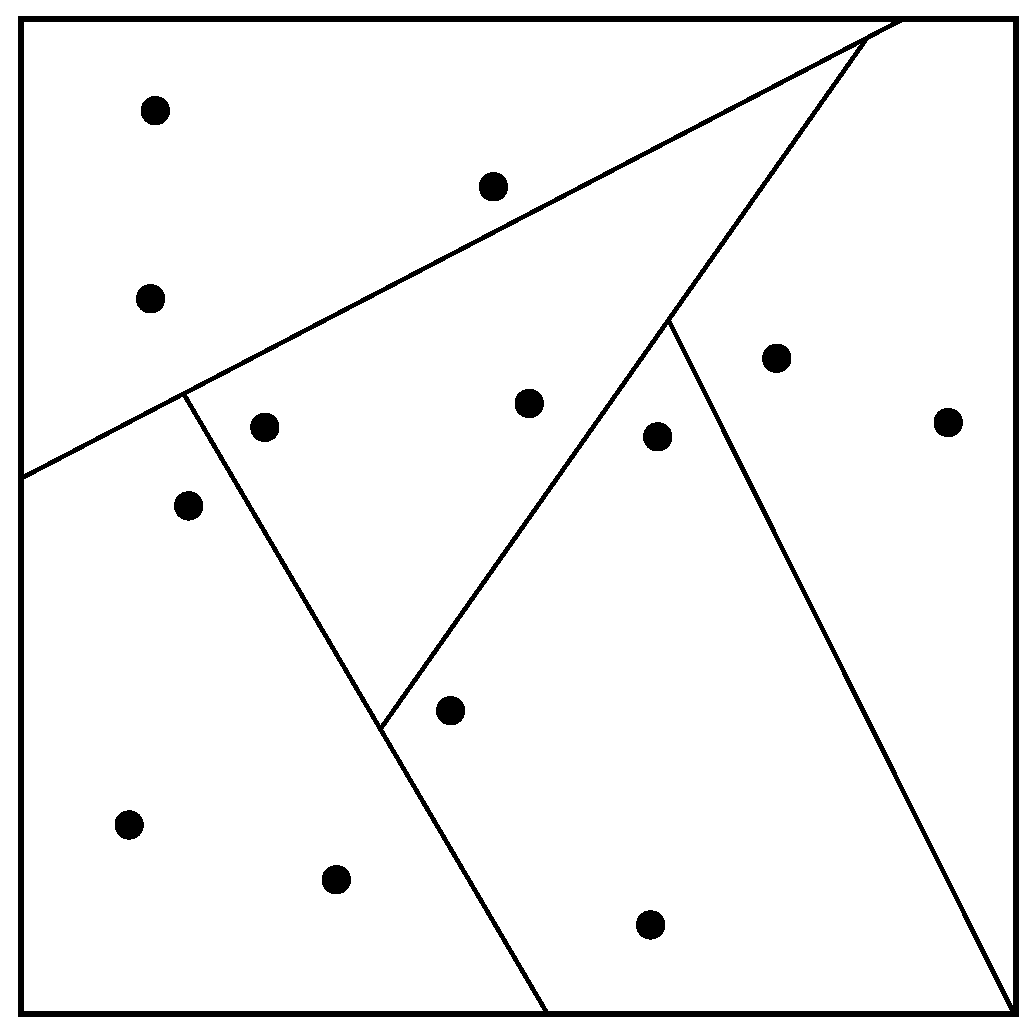
\includegraphics[width=0.5\linewidth]{images/bsp}
	\caption{Space partitioning using a BSP tree}
	\label{fig:bsp}
\end{figure}



\section{Proposed approach}
\label{sec:proposal}

The load balancing approach proposed by \cite{bezerra2009fgl} is based on two criteria: first, the system should be considered as potentially heterogeneous (i.e. every server may have a different amount of resources) and, second, the load on each server is \emph{not} proportional to the number of players connected to it, but to the amount of bandwidth required to send state update messages to them.

This choice is due to the fact that every player sends commands to the server at a constant rate, so the number of messages received by the server per unit time grows linearly with the number of players, whereas the number of state update messages sent by the server may be quadratic, in the worst case.

To divide the environment of the game into regions, it is proposed the utilization of a data structure known as kd-tree. The vast majority of MMOGs, such as World of Warcraft \cite{worldofwarcraft}, Ragnarok \cite{ragnarok} and \mbox{Lineage II} \cite{lineage2}, despite having three-dimensional graphics, the simulated world -- cities, forests, swamps and points of interest in general -- in these games is mapped in two dimensions. Therefore, we propose to use a kd-tree with \mbox{k = 2}.

Each node of the tree represents a region of the space and, moreover, in this node it is stored a split coordinate. Each one of the two children of that node represents a subdivision of the region represented by the parent node, and one of them represents the sub-region before the split coordinate and the other one, the sub-region containing points whose coordinates are greater than or equal to the split coordinate. The split axis (in the case of two dimensions, the axes $x$ and $y$) of the coordinate stored alternates for every level of the tree -- if the first level nodes store x-coordinates, the second level nodes store y-coordinates, the third level goes back to x-coordinates and so on. Every leaf node also represents a region of the space, but it does not store any split coordinate. Instead, it stores a list of the avatars present in that region. Finally, each leaf node is associated to a server of the game. When a server is overloaded, it triggers the load balancing, which uses the kd-tree to readjust the split coordinates that define its region, reducing the amount of content managed by it.

Every node of the tree also stores two other values: capacity and load of the subtree. The load of a non-leaf node is equal to the sum of the load of its children. Similarly, the capacity of a non-leaf node is equal to the sum of the capacity of its children nodes. For the leaf nodes, these values are the same of the server associated to each one of them. The tree root stores, therefore, the total weight of the game and the total capacity of the server system.

In the following sections, it will be described the construction of the tree, the calculation of the load associated with each server and the proposed balancing algorithm.

\subsection{Building the kd-tree}

To make an initial space division, it is constructed a balanced kd-tree. For this, it is used the recursive function shown in Algorithm \ref{alg:buildtree} to create the tree.

\begin{algorithm}
\caption{node::build\_tree(id, level, num\_servers)}
\label{alg:buildtree}
\begin{algorithmic}
	\IF{id + $2^{level} \ge num\_servers$ }
		\STATE $left\_child \leftarrow right\_child \leftarrow NIL$;
		\STATE return;
	\ELSE
		\STATE $left\_child \leftarrow$ new\_node();
		\STATE $left\_child.parent \leftarrow$ \textbf{this};
		\STATE $right\_child \leftarrow$ new\_node();
		\STATE $right\_child.parent \leftarrow$ \textbf{this};
		\STATE $left\_child$.build\_tree$(id, level + 1, num\_servers)$;
		\STATE $right\_child$.build\_tree$(id + 2^{level}, level + 1, num\_servers)$;
	\ENDIF
\end{algorithmic}
\end{algorithm}

\begin{figure}[!t]
	\centering
	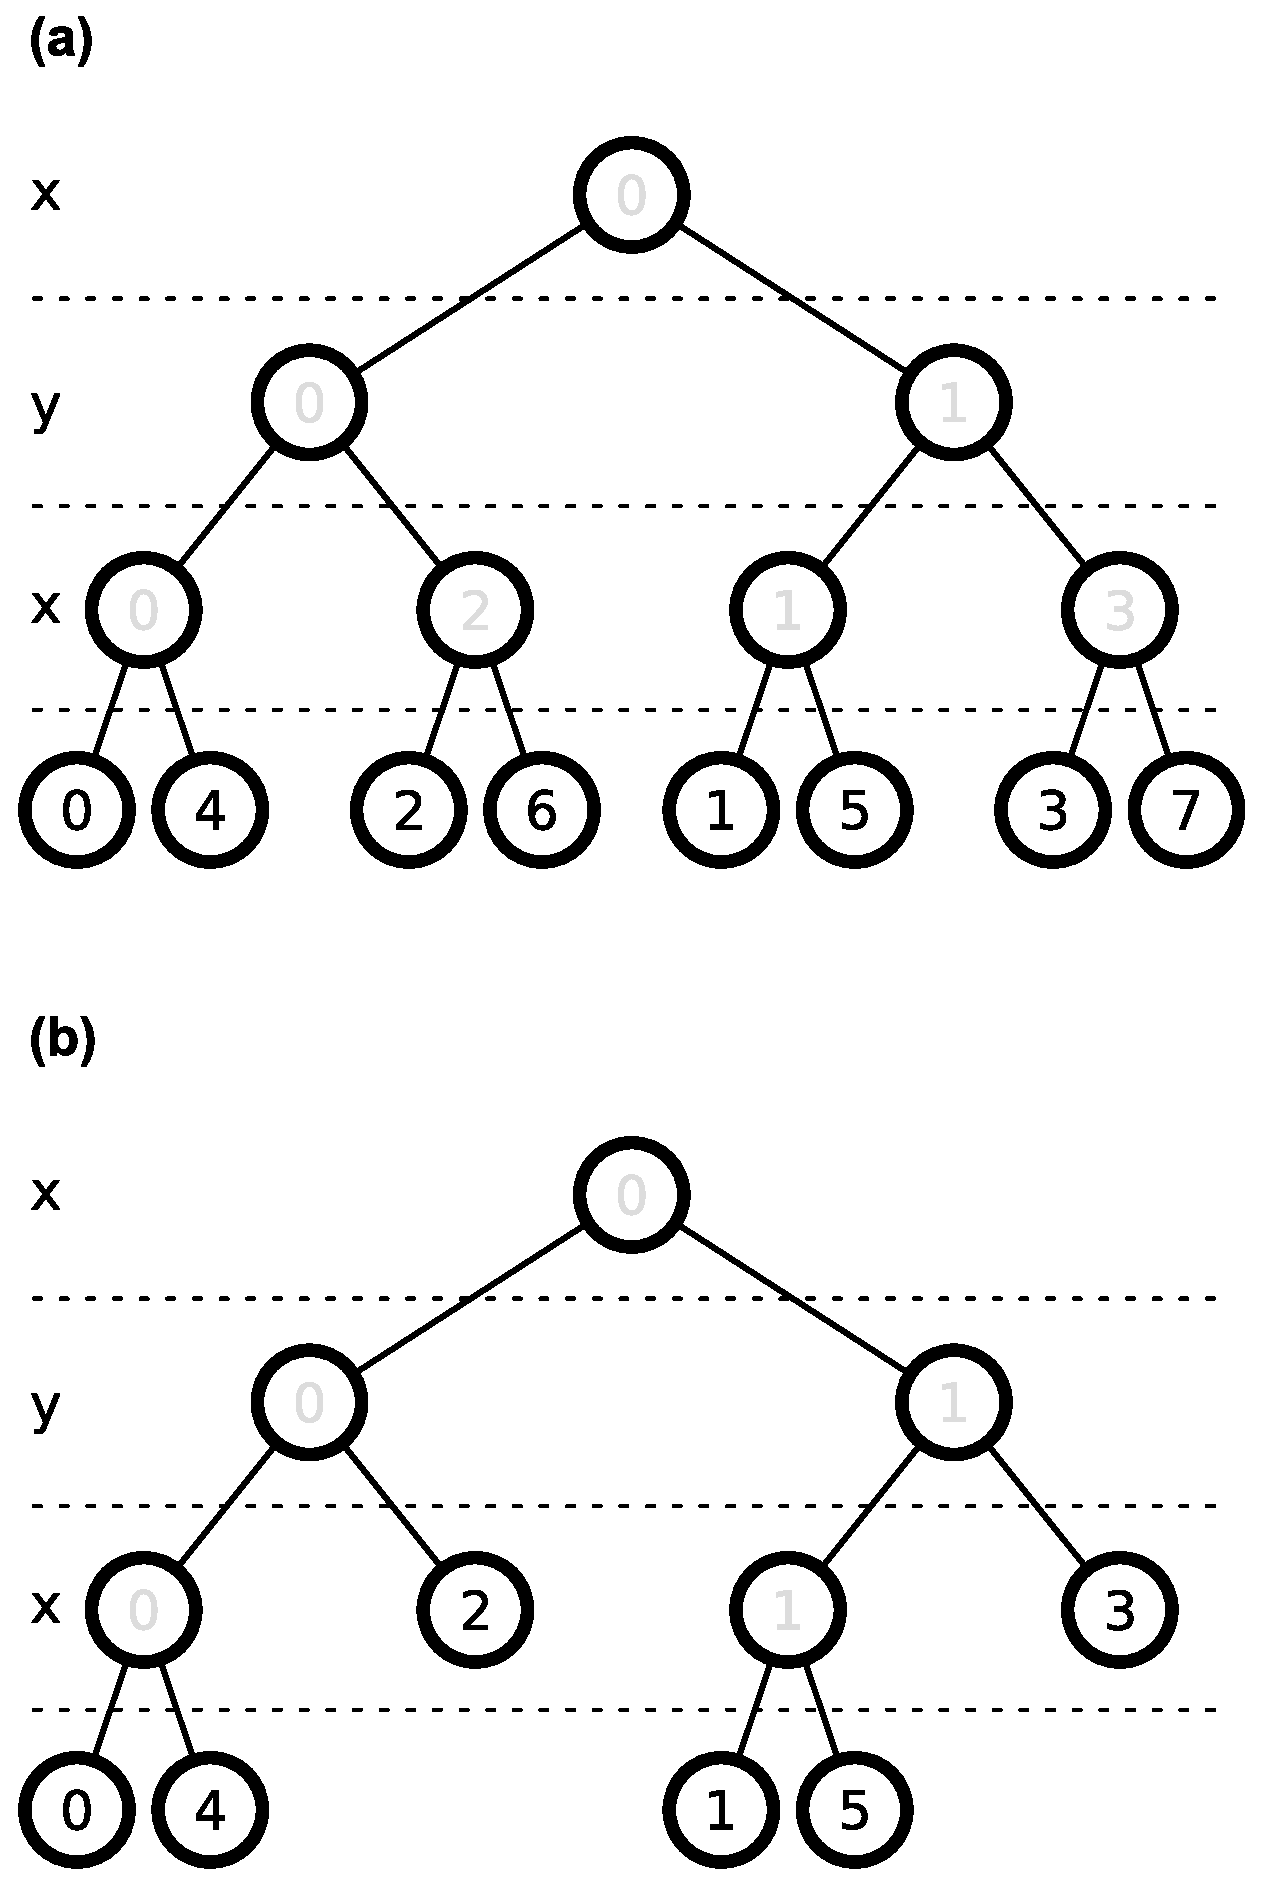
\includegraphics[width=0.75\linewidth]{images/kdtree}
	\caption{Balanced kd-trees built with the described algorithm}
	\label{fig:kdtree}
\end{figure}

In Algorithm \ref{alg:buildtree}, the $id$ value is used to calculate whether each node has children or not and, in the leaf nodes, it determines the server associated to the region represented by each leaf of the tree. The purpose of this is to create a balanced tree, where the number of leaf nodes on each of the two sub-trees of any node differs, in the maximum, by one. In Figure \ref{fig:kdtree} (a), we have a full kd-tree formed with this simple algorithm and, in Figure \ref{fig:kdtree} (b), an incomplete kd-tree with six-leaf nodes. As we can see, every node of the tree in (b) has two sub-trees whose number of leaf nodes differs by one in the worst case.

\subsection{Calculating the load of avatars and tree nodes}

The definition of the split coordinate for every non-leaf node of the tree depends on how the avatars will be distributed among the regions. An initial idea might be to distribute the players among servers, so that the number of players on each server is proportional to the bandwidth of that server. To calculate the split coordinate, it would be enough to simply sort the avatars in an array along the axis used ($x$ or $y$) by the tree node to split the space and, then, calculate the index in the vector, such that the number of elements before this index is proportional to the capacity of the left child and the number of elements from that index to the end of the array is proportional to the capacity of the right child (Figure \ref{fig:vector}). The complexity of this operation is $O(nlogn)$, due to the sorting of avatars.

\begin{figure}
  \centering
  \includegraphics[width=\linewidth]{images/vector}
  \caption{A load splitting considering only the number os avatars}
  \label{fig:vector}
\end{figure}

However, this distribution is not optimal, for the load imposed by the players depends on how they are interacting with one another. For example, if the avatars of two players are distant from each other, there will be probably no interaction between them and, therefore, the server will need only to update every one of them about the outcome of his own actions -- for these, the growth in the number of messages is linear with the number of players. On the other hand, if the avatars are close to each other, each player should be updated not only about the outcome of his own actions but also about the actions of every other player -- in this case, the number of messages may grow quadratically with the number of players \mbox{(Figure \ref{fig:load})}. For this reason, it is not sufficient only to consider the number of players to divide them among the servers.

\begin{figure}
  \centering
  \includegraphics[width=0.8\linewidth]{images/carga}
  \caption{Relation between avatars and load}
  \label{fig:load}
\end{figure}

A more appropriate way to divide the avatars is by considering the load imposed by each one of them on the server. A brute-force method for calculating the loads would be to get the distance separating each pair of avatars and, based on their interaction, calculate the number of messages that each player should receive by unit of time. This approach has complexity $O(n^2)$. However, if the avatars are sorted according to their coordinates on the axis used to divide the space in the kd-tree, this calculation may be performed in less time.

For this, two nested loops are used to sweep the avatars array, where each of the avatars contains a $load$ variable initialized with zero. As the vector is sorted, the inner loop may start from an index before which it is known that no avatar $a_j$ has relevance to that being referenced in the outer loop, $a_i$. It is used a variable $begin$, with initial value of zero: if the coordinate of $a_j$ is smaller than that of $a_i$, with a difference greater than the maximum view range of the avatars, the variable $begin$ is incremented. For every $a_j$ which is at a distance smaller than the maximum view range, the $load$ of $a_i$ is increased according to the relevance of $a_j$ to $a_i$. When the inner loop reaches an avatar $a_j$, such that its coordinate is greater than that of $a_i$, with a difference greater than the view range, the outer loop moves immediately to the next step, incrementing $a_i$ and setting the value of $a_j$ to that stored in $begin$ (Figure \ref{fig:sweep}).

Let $width$ be the length of the virtual environment along the axis used for the splitting; let also $radius$ be the maximum view range of the avatars, and $n$, the number of avatars. The number of relevance calculations, assuming that the avatars are uniformly distributed in the virtual environment is \mbox{$O(m \times n)$}, where $m$ is the number of avatars compared in the internal loop, i.e. \mbox{$m = \frac{2 \times radius \times n}{width}$}. The complexity of sorting the avatars along one of the axes is $O(nlogn)$. Although it is still quadratic, the execution time is reduced significantly, depending on the size of the virtual environment and on the view range of the avatars. The algorithm could go further and sort each set of avatars $a_j$ which are close (in one of the axes) to $a_i$ according to the other axis and, again, perform a sweep eliminating those which are too far away, in both dimensions. The number of relevance calculations would be \mbox{$O(p \times n)$}, where $p$ is the number of avatars close to $a_i$, considering the two axes of coordinates, i.e. \mbox{$p = \frac{(2 \times radius)^2 \times n}{width \times height}$}. In this case, $height$ is the extension of the environment in the second axis taken as reference. Although there is a considerable reduction of the number of relevance calculations, it does not pay the time spent in sorting the sub-array of the avatars selected for each $a_i$. Adding up all the time spent on sort operations, it would be obtained a complexity of: \mbox{$O(nlogn + n \times mlogm)$}.

\begin{figure}
  \centering
  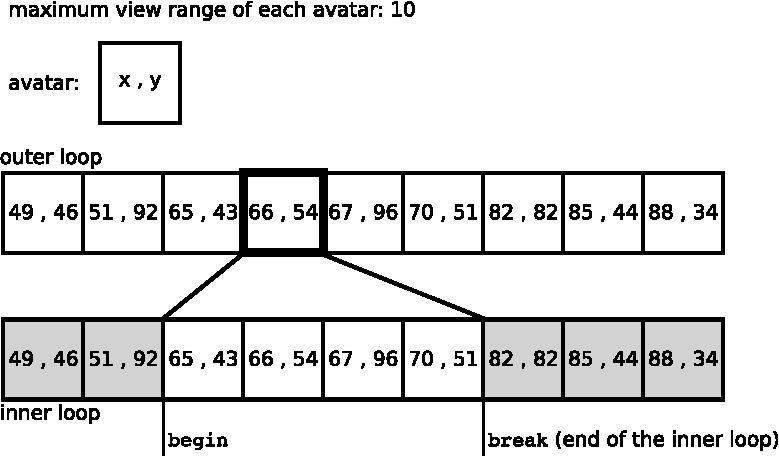
\includegraphics[width=0.8\linewidth]{images/sweep}
  \caption{Sweep of the sorted array of avatars}
   \label{fig:sweep}
\end{figure}

After calculating the load generated by each avatar, this value is used to define the load on each leaf node and, recursively, on the other nodes of the kd-tree. To each leaf node a server and a region of the virtual environment are assigned. The load of the leaf node is equal to the server's bandwidth used to send state updates to the players controlling the avatars located in its associated region. This way, the load of each leaf node is equal to the sum of the weights of the avatars located in the region represented by it.

\subsection{Dynamic load balancing}

Once the tree is built, each server is associated to a leaf node -- which determines a region. All the state update messages to be sent to players whose avatars are located in a region must be sent by the corresponding server. When a server is overloaded, it may transfer part of the load assigned to it to some other server. To do this, the overloaded server collects some data from other servers and, using the kd-tree, it adjusts the split coordinates of the regions.

Every server maintains an array of the avatars located in the region managed by it, sorted according to the $x$ coordinate. Also, each element of the array stores a pointer to another element, forming a chained list that is ordered according to the $y$ coordinated of the avatars (Figure \ref{fig:vectorxlisty}). By maintaining a local sorted avatar list on each server, the time required for balancing the load is somewhat reduced, for there will be no need for the server performing the rebalance to sort again the avatar lists sent by other servers. It will need only to merge all the avatars lists received from the other servers in an unique list, used to define the limits of the regions, what is done by changing the split coordinates which define the space partitions.

\begin{figure}
  \centering
  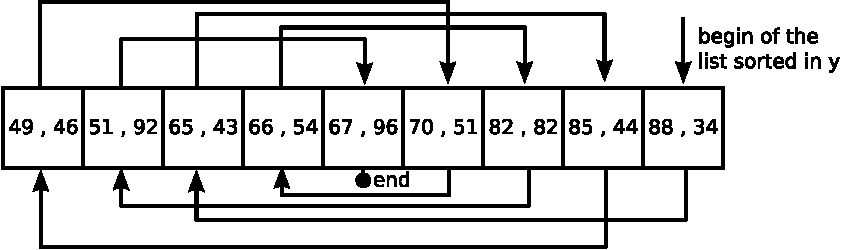
\includegraphics[width=0.9\linewidth]{images/vectorxlisty}
  \caption{Avatar array sorted by x, containing a list sort by y}
   \label{fig:vectorxlisty}
\end{figure}

When the overloaded server initiates the rebalance, it runs an algorithm that traverses the kd-tree, beginning from the leaf node that defines its region and going one level up at each step until it finds an ancestor node with a capacity greater then or equal to the load. While this node is not found, the algorithm continues recursively up the tree until it reaches the root. For each node visited, a request for the information about all the avatars and the values of load and capacity is sent to the servers represented by the leaf nodes of the sub-tree to the left of that node (Figure \ref{fig:ancestors}). With these data, and its own list of avatars and values of load and capacity, the overloaded server can calculate the load and capacity of its ancestral node visited in the kd-tree, which are not known beforehand -- these values are sent on-demand to save up some bandwidth of the servers and to keep the system scalable.

\begin{figure}
  \centering
  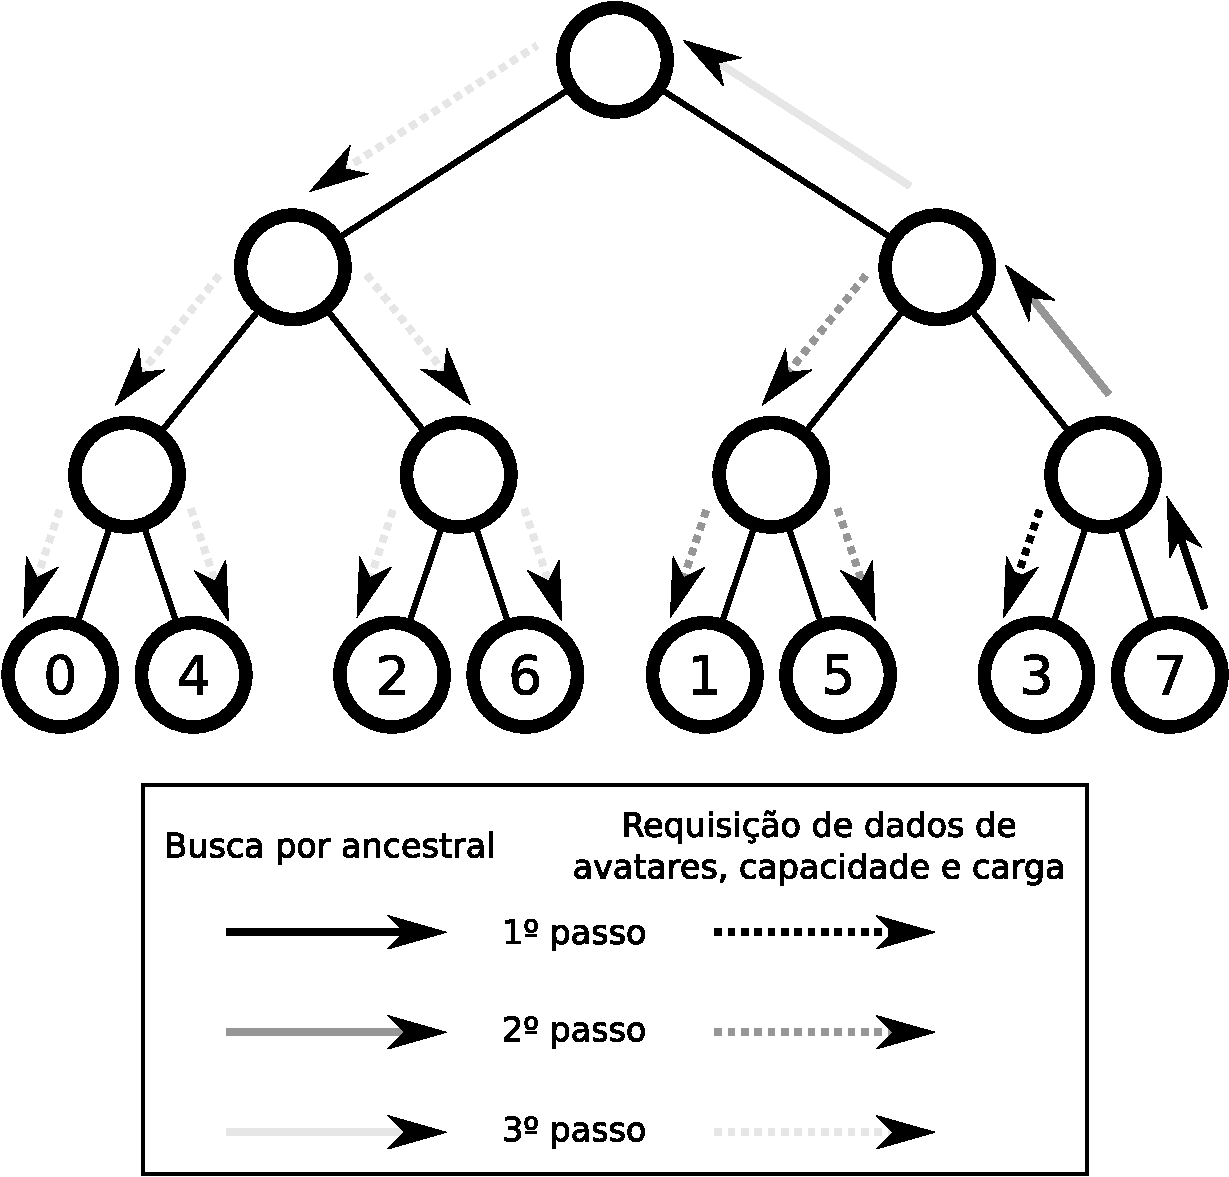
\includegraphics[width=0.9\linewidth]{images/ancestors}
  \caption{Search for an ancestor node with enough resources}
   \label{fig:ancestors}
\end{figure}

Reaching an ancestral node with capacity greater than or equal to the load -- or the root of the tree, if no such node is found -- the server that initiated the balance adjusts the split coordinates of the kd-tree nodes. For each node, it sets the split coordinate in a way such that the avatars are distributed according to the capacity of the node's children. For this, it is calculated the load fraction that should be assigned to each child node. The avatar list is then swept, stopping at the index $i$ such that the total load of the avatars before $i$ is approximately equal to the value defined as the load to be designated to the left child of the node whose split coordinate is being calculated (Figure \ref{fig:balancenode}). The children nodes have also, in turn, their split coordinates readjusted recursively, so that they are checked for validity -- the split coordinate stored in a node must belong to the region defined by its ancestors in the kd-tree -- and readjusted to follow the balance criteria defined.

\begin{figure}
  \centering
  \includegraphics[width=0.9\linewidth]{images/balancenode}
  \caption{Division of an avatar list between two brother nodes}
   \label{fig:balancenode}
\end{figure}

As the avatar lists received from the other servers are already sorted along both axes, it is enough to merge these structures with the avatar list of the server which initiated the rebalance. Assuming that each server already calculated the weight of each avatar managed by it, the rebalance time is  $O(nlogS)$, where $n$ is the number of avatars in the game and $S$ is the number of servers. The communication cost is $O(n)$, caused by the sending of data related to te $n$ avatars. The merging of all avatar lists has $O(n)$ complexity, for the avatars were already sorted by the servers. At each level of the kd-tree, $O(n)$ avatars are swept in the worst case, in order to find the $i$ index whose avatar's coordinate will be used to split the regions defined by each node of the tree (Figure \ref{fig:balancenode}). As this is a balanced tree with $S$ leaf nodes, it has a height of $\lceil logS \rceil$.



\section{Work analysis}

In this chapter, we presented a work where \cite{bezerra2009fgl} propose the use of a kd-tree to partition the virtual environment of MMOGs and perform the load balancing of servers by recursively adjusting the split coordinates stored in its nodes. One of the conclusions reached was that the use of kd-trees to make this partitioning allows a finer granularity of the load distribution, while the readjustment of the regions becomes simpler -- by recursively traversing the tree -- than the common approaches, based on cells and/or graph partitioning.

The finer granularity allows for a better balancing, so that the load assigned to each server is close to the ideal value that should be assigned to it. This better balance also helps to reduce the number of migrations, for it can perform less rebalancing operations to achieve the same distribution fairness. The fact that the regions defined by the kd-tree are necessarily contiguous also contribute to a lower number of migrations of players between servers.

It was also possible to use methods with a lower complexity for each rebalancing operation. This is due, first, to the reduction of the number of operations for calculating the relevance between pairs of avatars by sweeping a sorted avatar list and, secondly, to keeping at each server an avatar list already sorted in both dimensions, saving the time that would be spent on sorting the avatars when they were received by the server executing the rebalance.

This approach, however, has a serious limitation: the split axes are always parallel to the $x$ and $y$ axes. That may lead, sometimes, to a worse division of the players among servers, as each region is necessarily a rectangle with its sided aligned to the coordinates axes. Also, each server has an indivisible and contiguous region assigned to it. Although this may reduce the number of player migrations, a fragmented region could be of use sometimes, adding some flexibility to the world partitioning.